\documentclass[12pt]{article} % article - typ/šablona dokumentu
\usepackage[czech]{babel} % nastavuje české popisky např. u obsahu, referencí, tabulek, obázků 
\usepackage[utf8]{inputenc} % použito UTF8 kvůli češtině (zvládá prakticky všechny jazyky na světě)

\begin{document}
	Hello world!
	$a^2+b^2=c^2$ %math mode
	Ahoj světe!
\end{document}
% vše co je za "\end{document}" se již nezpracovává (neobjeví ve výsledném dokumentu)

% vše co je za procentem LaTeX ignoruje (bere jako komentář)


% ---------------------------
% nová stránka
\newpage
% ---------------------------

% ---------------------------
% úvodní stránka
\begin{titlepage}

\begin{center}
  \Huge
  \textsc{Dům dětí a mládeže Brno, Helceletova\\
  \huge Pobočka Robotárna\\}
  \vspace{\stretch{0.382}}
  \LARGE
  Jak a proč používat \LaTeX\\
  \Huge
  \vspace{\stretch{0.618}}
\end{center}

{\Large \today \hfill
Jarek Páral, Vojtěch Boček}
\end{titlepage}
% ---------------------------

% ---------------------------
% kapitoly/sekce
\section{Kapitola 1}

Lorem ipsum dolor sit amet, consectetur adipiscing elit. Proin tincidunt mollis nisl, in finibus dolor accumsan ultricies. Integer consectetur purus eu lacus sodales consectetur. Donec fermentum lacinia mi, ac malesuada nisi convallis in. Phasellus aliquam quam elit, hendrerit feugiat nunc pulvinar non. Aliquam vestibulum in sapien ut dapibus.

\subsection{Podkapitola 1.1}

Lorem ipsum dolor sit amet, consectetur adipiscing elit. Proin tincidunt mollis nisl, in finibus dolor accumsan ultricies. Integer consectetur purus eu lacus sodales consectetur. Donec fermentum lacinia mi, ac malesuada nisi convallis in. Phasellus aliquam quam elit, hendrerit feugiat nunc pulvinar non. Aliquam vestibulum in sapien ut dapibus.

\subsubsection{Podpodkapitola 1.1.1}

Lorem ipsum dolor sit amet, consectetur adipiscing elit. Proin tincidunt mollis nisl, in finibus dolor accumsan ultricies. Integer consectetur purus eu lacus sodales consectetur. Donec fermentum lacinia mi, ac malesuada nisi convallis in. Phasellus aliquam quam elit, hendrerit feugiat nunc pulvinar non. Aliquam vestibulum in sapien ut dapibus.
% ---------------------------

% ---------------------------
% obsah
\tableofcontents
% ---------------------------

% ---------------------------
% obrázky
% ---------------------------
% potřeba vložit před "\begin{document}"
\usepackage{graphicx} % pro vkládání obrázků a příkaz "\includegraphics"
% ---------------------------
% samotné vložení obrázku
\begin{figure}[t]
	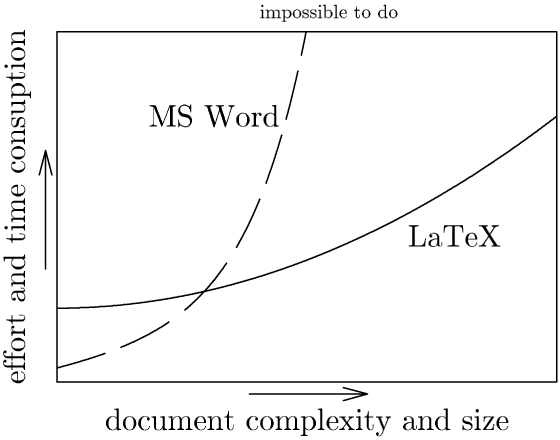
\includegraphics[width=\textwidth]{../img/when_use_latex.png}
	\caption{Kdy se vyplatí použít \LaTeX} % popis, který se zobrazí pod obrázkem
	\label{moje_navesti} %identifikuje objekt, který lze pak referencovat
\end{figure}
% ---------------------------


% ---------------------------
% poznámky pod čarou
Text u kterého bude index\footnote{text, který bude pod čarou}, text za poznámkou/indexem 
% ---------------------------

% ---------------------------
% odkazy v textu
% návěští na odkazovaný objekt - přidejte např. k obrázku/tabulce
\label{moje_navesti} %identifikuje objekt

Tohle je reference/odkaz na daný obrázek/tabulku. Příklad: Obrázek \ref{moje_navesti} popisuje kdy se vyplatí používat \LaTeX
% ---------------------------

% ---------------------------
% matematika v textu
 $a^2+b^2=c^2$ 
% ---------------------------

% ---------------------------
% matematika v samostatném bloku
% ---------------------------
% potřeba vložit před "\begin{document}" pro fungování matematiky
\usepackage{amsmath}
\usepackage{amsthm}
\usepackage{amsfonts}
% --------------------------
% nečíslovaná rovnice (způsobuje hvězdička za equation)
\begin{equation*}
\lim_{x \to \infty}\frac{\sin^2 x + \cos^2 x}{4} = y \nonumber
\end{equation*}	

% číslovaná rovnice (nemá hvězdičku za equation)
\begin{equation}
\int_a^b f(x) \mathrm{d}x = -\int_b^a f(x) \mathrm{d}x 
\end{equation}
% ---------------------------

% ---------------------------
% seznam obrázků
\listoffigures %seznam obrázků	
% ---------------------------

% ---------------------------
% seznam tabulek
\listoftables %seznam tabulek
% ---------------------------

% ---------------------------
% číselné a odrážkového seznamy
% ---------------------------
% potřeba vložit před "\begin{document}"
\usepackage{enumerate} % číselné seznamy
% ---------------------------
 \begin{enumerate}
   \item první číslovaná položka
     \begin{enumerate}
       \item první číslovaná pod položka
       \item druha číslovaná pod položka
     \end{enumerate}
   \item druha položka
     \begin{itemize}
       \item první pod odrážka
       \item druha pod odrážka
     \end{itemize}
 \end{enumerate}
% ---------------------------

% ---------------------------
% tabulka
\begin{table}[h]
  \begin{center}
  \catcode`\-=12
    \begin{tabular}{|c|c|} \hline
      $A$ & $\neg A$\\ \hline
      \textbf{P} & N\\ \hline
      \textbf{O} & O\\ \hline
      \textbf{X} & X\\ \hline
      \textbf{N} & P\\ \hline
    \end{tabular}
    \begin{tabular}{|c|c|c|c|c|c|} \hline
      \multicolumn{2}{|c|}{} & \multicolumn{4}{|c|}{$B$}\\ \cline{3-6}
      \multicolumn{2}{|c|}{A $\wedge$ B} & \textbf{P} & \textbf{O} & \textbf{X} & \textbf{N}\\ \hline
                            & \textbf{P} & P & O~& X & N\\ \cline{2-6}
                            & \textbf{O} & O~& O~& N & N\\ \cline{2-6}  
                          A~& \textbf{X} & X & N & X & N\\ \cline{2-6}
                            & \textbf{N} & N & N & N & N\\ \hline
    \end{tabular}
    \begin{tabular}{|c|c|c|c|c|c|} \hline
      \multicolumn{2}{|c|}{} & \multicolumn{4}{|c|}{$B$}\\ \cline{3-6}
      \multicolumn{2}{|c|}{A $\vee$ B} & \textbf{P} & \textbf{O} & \textbf{X} & \textbf{N}\\ \hline
                            & \textbf{P} & P & P & P & P\\ \cline{2-6}
                            & \textbf{O} & P & O~& P & O\\ \cline{2-6}
                        A~& \textbf{X} & P & P & X & X\\ \cline{2-6}
                            & \textbf{N} & P & O~& X & N\\ \hline
    \end{tabular}
    \begin{tabular}{|c|c|c|c|c|c|} \hline
      \multicolumn{2}{|c|}{} & \multicolumn{4}{|c|}{$B$}\\ \cline{3-6}
      \multicolumn{2}{|c|}{A $\rightarrow$ B} & \textbf{P} & \textbf{O} & \textbf{X} & \textbf{N}\\ \hline
                            & \textbf{P} & P & O~& X & N\\ \cline{2-6}
                            & \textbf{O} & P & O~& P & O\\ \cline{2-6}
                         A~& \textbf{X} & P & P & X & X\\ \cline{2-6}
                            & \textbf{N} & P & P & P & P\\ \hline
    \end{tabular}
    \caption{Protože Kleeneho trojhodnotová logika už je "zastaralá", uvádíme si zde příklad čtyřhodnotové logiky}
    \label{tab2}
  \end{center}
\end{table}
% ---------------------------



